\documentclass[a4paper,12pt]{report}
\usepackage[toc,page]{appendix}
\usepackage{amsmath}
\usepackage{float}
\usepackage{graphicx}
\usepackage{subfig}
\usepackage{amssymb}
\usepackage{geometry}
\usepackage{array}
\usepackage{tcolorbox}
\usepackage[normalem]{ulem}

\usepackage{setspace}
 \geometry{
 a4paper,
 total={170mm,257mm},
 left=20mm,
 top=20mm,
 }
\usepackage{tikz}
\usepackage{pgfplots}
\usetikzlibrary{shapes, arrows.meta, decorations.pathreplacing, positioning, petri, fit, calc}
\tikzstyle{startstop} = [circle, minimum size=1cm ,text centered, draw=black]
\tikzstyle{neuron} = [circle, minimum size=1cm ,text centered, draw=red, fill=gray!30]
\tikzstyle{neuronEll} = [ellipse, minimum size=1cm ,text centered, text width=2cm, draw=red, fill=gray!30]
\tikzstyle{process} = [rectangle, minimum width=2cm, minimum height=0.5cm, text centered, text width=3cm, draw=black, fill=blue!30]
\tikzstyle{detail} = [rectangle, minimum width=1.5cm, minimum height=0.5cm, text justified, text width=2.6cm, fill=white!30]
\tikzstyle{smalldetail} = [rectangle, minimum width=2cm, minimum height=1cm, text centered, text width=2cm]
\tikzstyle{largedetail} = [rectangle, minimum width=3cm, minimum height=1cm, text centered, text width=4cm, fill=white!30]
\tikzstyle{box} = [rectangle, minimum width=5cm, minimum height=9cm, text centered, text width=4cm, draw=black, fill=white!30]

\usepackage[utf8]{inputenc}

% Default fixed font does not support bold face
\DeclareFixedFont{\ttb}{T1}{txtt}{bx}{n}{10} % for bold
\DeclareFixedFont{\ttm}{T1}{txtt}{m}{n}{10}  % for normal

% Custom colors
\usepackage{color}
\definecolor{deepblue}{rgb}{0,0,0.5}
\definecolor{deepred}{rgb}{0.6,0,0}
\definecolor{deepgreen}{rgb}{0,0.5,0}

\usepackage{listings}

% Python style for highlighting
\newcommand\pythonstyle{\lstset{
language=Python,
basicstyle=\ttm,
otherkeywords={self},             % Add keywords here
keywordstyle=\ttb\color{deepblue},
emph={MyClass,__init__},          % Custom highlighting
emphstyle=\ttb\color{deepred},    % Custom highlighting style
stringstyle=\color{deepgreen},
frame=tb,                         % Any extra options here
showstringspaces=false            % 
}}


% Python environment
\lstnewenvironment{python}[1][]
{
\pythonstyle
\lstset{#1}
}
{}

% Python for external files
\newcommand\pythonexternal[2][]{{
\pythonstyle
\lstinputlisting[#1]{#2}}}

% Python for inline
\newcommand\pythoninline[1]{{\pythonstyle\lstinline!#1!}}


\begin{document}
\tableofcontents

\title{Clustering algorithm: Unsupervised Learning}
\maketitle
\part{Week 8}
\section{Supervised Learning vs. Unsupervised Learning}
\begin{itemize}
	\item \textbf{Supervised Learning} $\rightarrow$ Training set is of the form:\\
	\begin{align*}
		\left[(x^{(1)}, y^{(1)}), (x^{(2)}, y^{(2)}), ....(x^{(m)}, y^{(m)}) \right]
	\end{align*}
	\item \textbf{Unsupervised Learning} $\rightarrow$ Training set is of the form (no labels $y$):\\
	\begin{align*}
		\left[ x^{(1)}, x^{(2)},....,x^{(m)} \right]
	\end{align*} 
\end{itemize}

\begin{figure}[H]
	\centering
        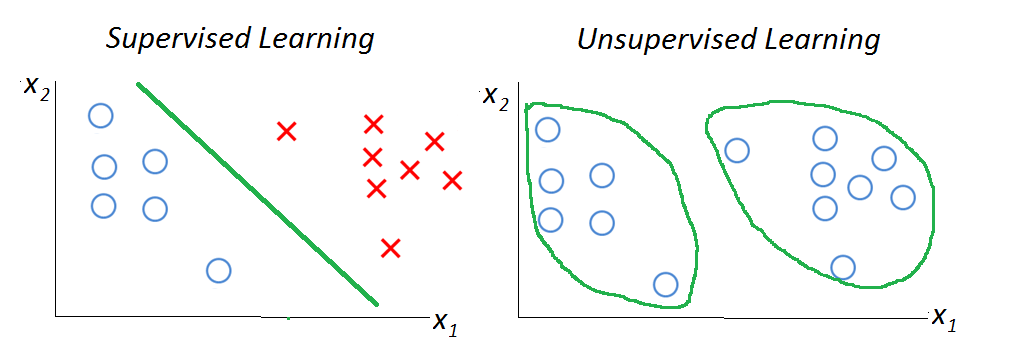
\includegraphics[totalheight=4 cm]{fig1.png}
\end{figure}


\section{Clustering algorithm: $K$-means}
	\subsection{Principle}
$K-$means is a iterative algorithm:

\begin{enumerate}
	\item inputs:
		\begin{itemize}
			\item	$K$: number of clusters that we want to find in the data set
			\item Training set: $\left[x^{(1)}, x^{(2)}, ....x^{(m)} \right]$ where $x^{(i)} \in \mathbb{R}^n$ (by convention, $x_0=1$ is dropped).
		\end{itemize}
	\item Randomly initialize (set the location) of $K$ cluster centroids: $\mu_1, \mu_2, \mu_3, ...., \mu_K \in \mathbb{R}^n$. \\
	\item Algorithm:\\
\begin{tcolorbox}
\begin{python}
Repeat {
	1) Cluster assignment step: 
	Go thru each example and assign them to the closest 
	cluster centroid
	for i = 1 to m:
		c[i] := index (1 to K) of cluster centroid closest to x[i]
	end
		
	2) Move centroid step: 
	Take the mean of all points associated with a cluster
	and move the centroid to that new position. 
	for i = 1 to K:
		mu[k] := mean of points assigned to cluster k
	end	
	Reiterate until convergence==>	
\end{python}
\end{tcolorbox}
\item Mathematically:
\begin{itemize}
\item In the cluster assignment step, c[i] ($c^{(i)}$) is the value of $k$ that minimizes $||x^{(i)} - \mu_k ||^2$ 
			($J$ is minimized with respect to all $c^{(i)}$, while holding all $\mu_k$ fixed)
\item In the 'move centroid step', $J$ is minimized with respect to all $\mu_k$, and holding all $c^{(i)}$ fixed
\end{itemize}
\end{enumerate}
\begin{itemize}
\item Example: Let's consider $x^{(1)}$, $x^{(5)}$, $x^{(6)}$, $x^{(10)}$, and assign them to cluster 2 ($\mu_2$). Therefore: $c^{(1)} = 2$, $c^{(5)} = 2$, $c^{(6)} = 2$, $c^{(10)} = 2$. The new position of $\mu_2$ is: \\
$\mu_2 = \frac{1}{4} \left[x^{(1)} + x^{(5)}  + x^{(6)}  + x^{(10)}  \right] (\in \mathbb{R}^n)$
\end{itemize}

\begin{figure}[H]
	\centering
        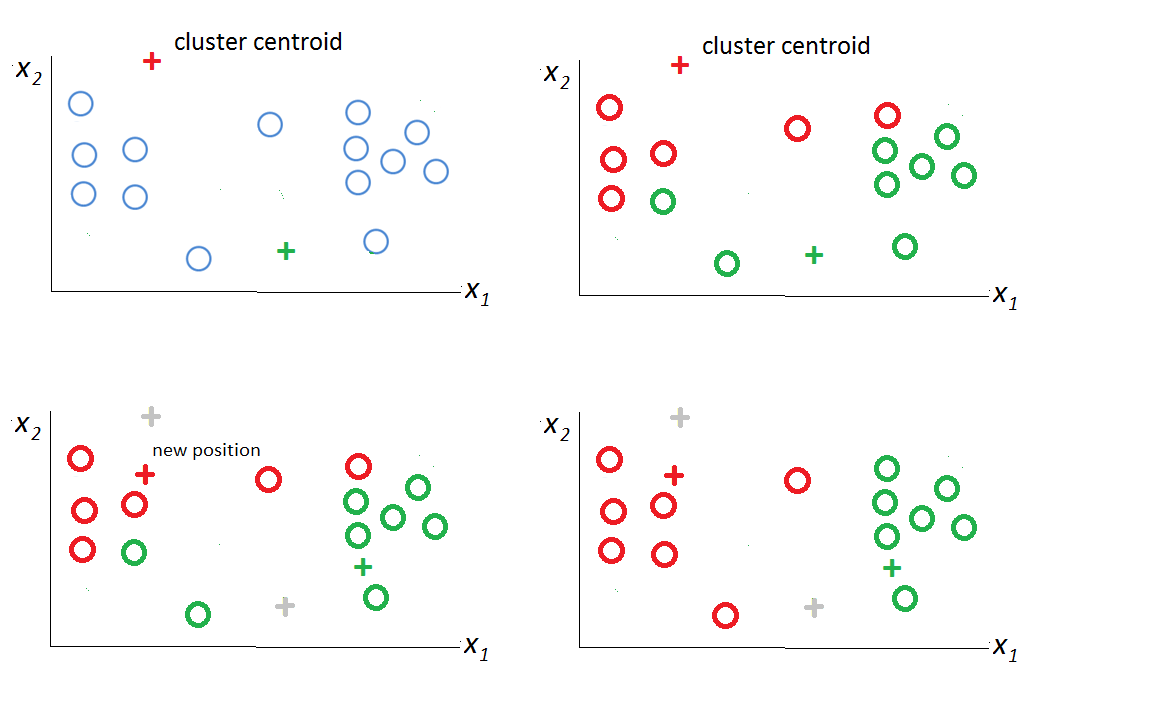
\includegraphics[totalheight=6 cm]{fig2.png}\caption{Illustration of the K-means algorithm}
\end{figure}


\begin{itemize}
\item Note: if a cluster cannot find any points to assign, by convention the cluster is eliminated.
\end{itemize}

\section{Optimization Objective}
\begin{itemize}
\item $c^{(i)}$ is the index of cluster (1, 2,...,$K$) to which example $x^{(i)}$ is currently assigned.
\item $\mu_k$ = cluster centroid $k$ ($\mu_k \in \mathbb{R}^n$ with $k \in \{1,2, ..., K \}$)
\item $\mu_{c^{(i)}}$ = cluster centroid of the cluster to which example $x^{(i)}$ has been assigned \\
$x^{(1)} \rightarrow 5  \Rightarrow C^{(i)} = 5 \rightarrow \mu_{c^{(i)}} = \mu_5$ \\
 
\item \textbf{Optimization objective} :\\
\begin{align}
J(c^{(1)}, ...c^{(m)}, \mu_1, \mu_2,..., \mu_k) = \frac{1}{m} \sum_{i=1} ^m ||x^{(i)}- \mu_{c^{(i)}}||^2
\end{align}
This cost function is sometimes called 'Distorsion'. \\
\item \textbf{Cost function minimization}:
\begin{align}
min_{\stackrel{c^{(1)}, ...c^{(m)}}{\mu_1, \mu_2,..., \mu_k}, } J \left(c^{(1)}, ...c^{(m)}, \mu_1, \mu_2,..., \mu_k \right)
\end{align}
\end{itemize}

\section{Random Initialization of cluster centroid}
\begin{itemize}
\item Should have $K < m$
\item Randomly pick $K$ \textbf{training examples} and set $\mu_1, \mu_2, ...\mu_K$ equals to those K examples: \\
$\mu_1 = x^{(i)}$, $\mu_2 = x^{(j)}$ where $i, j$ random. \\
\item Local optimum: Depending on the initialization, $K-$means can converge to different solution (the distorsion function could be trapped in local optimum). One method is to try multiple random initialization\\
\end{itemize}

\begin{tcolorbox}
\begin{python}
for i = 1 to 100 
	randomly initialize K-means
	Run $K-$means and get c[1], ...c[m], mu[1], ...,mu[k] \\
	Compute cost  function distorsion
end
Pick clustering that gives the lowest cost.
\end{python}
\end{tcolorbox}
Additional notes:

\begin{itemize}
\item for small Nbrs of clusters, doing multiple Random Initialization helps in giving good clustering.
\item If $K>10$, multiple clustering is less likely to give better solution.
\end{itemize}
\section{Choose the Number of Clusters $K$}
One known method to determine an appropriate cluster size is the 'Elbow Method', where the optimum cluster size is given by the Elbow of $J$ versus $k$.
However, in reality, the curve $J(k)$ rarely show a clear a elbow feature.
\begin{figure}[H]
	\centering
        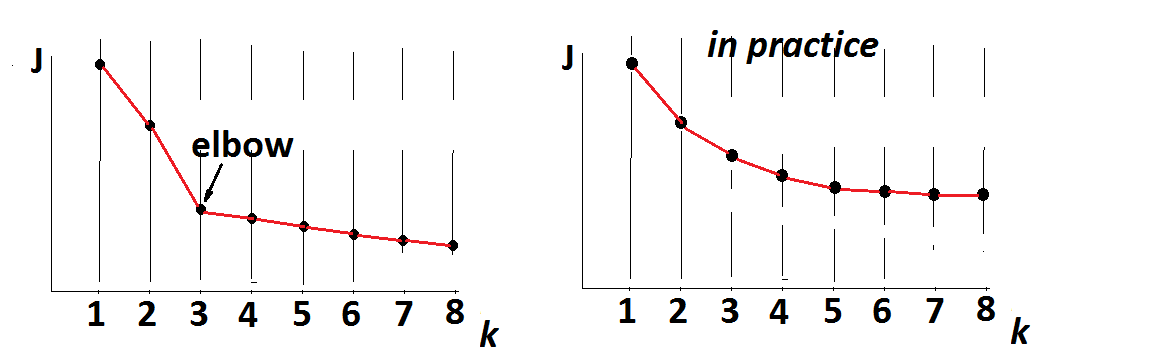
\includegraphics[totalheight=5 cm]{fig4.png}\caption{Illustration of the K-means algorithm}
\end{figure}

\section{Dimensionality Reduction}
Dimensionality reduction enables to run algorithm more quickly. For highly correlated dimensions, it is useful to perform Dimensionality Reduction.
\begin{figure}[H]
	\centering
        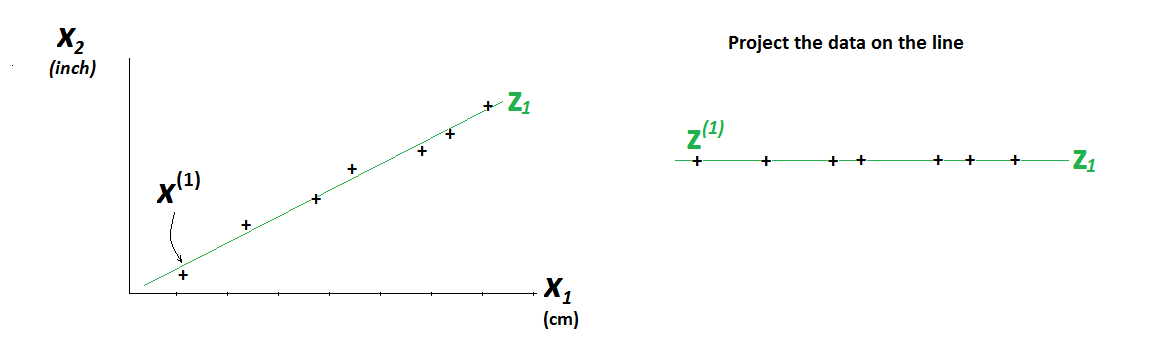
\includegraphics[totalheight=5 cm]{fig5.png}\caption{Illustration of dimensionality reduction 2D to 1D. }
\end{figure}

\begin{itemize}
\item Dimensiontionality reduction 2D to 1D:
\begin{align}
x^{(1)}, ..., x^{(m)} \in \mathbb{R}^2 \Rightarrow z^{(1)}, ..., z^{(m)} \in \mathbb{R}
\end{align}
\item Dimensiontionality reduction 3D to 2D:
\begin{align}
x^{(1)}, ..., x^{(m)} \in \mathbb{R}^3 \Rightarrow z^{(1)}, ..., z^{(m)} \in \mathbb{R}^2
\end{align}
\end{itemize}


\subsection{Data Visualization}
Dimensionality reduction from n-dimension to 2 dimensions is performed to visualize the data. 

\subsection{Principal Component Analysis (PCA) algorithm}
PCA is used for dimensionality reduction.
\begin{enumerate}
\item Training set: $x^{(1)}$, ...., $x^{(m)}$
\item Always normalization:
\begin{align}
\mu_j = \frac{1}{m} \sum_{i=1} ^m x_j ^{(i)}
\end{align}
and replace each $x_j ^{(i)} \leftarrow (x_j ^{(i)}- \mu_j)$
\item Feature scaling \\
and replace each $x_j ^{(i)} \leftarrow \frac{(x_j ^{(i)}- \mu_j)}{s_j}$, where $s_j$ is the standard deviation.
\item PCA tries to find a lower dimensional surface/line onto which the projection error is minimized.
\end{enumerate}
\begin{figure}[H]
	\centering
        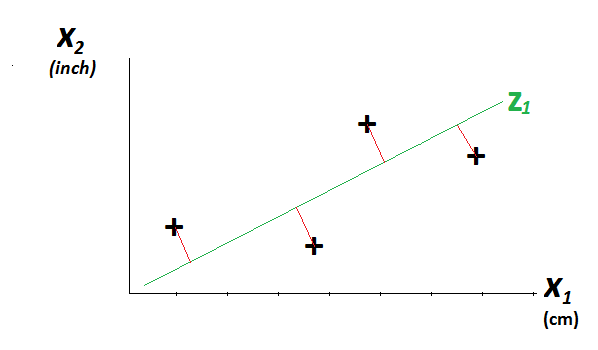
\includegraphics[totalheight=6 cm]{fig6.png}\caption{}
\end{figure}
\subsubsection{Formulation}
\begin{itemize}
\item Dimensiontionality reduction n-D to k-D: Find k direction vectors ($u^{(1)},...,u^{(k)} $) onto which to project the data, so as to minimize the projection error.\\
\item PCA is not linear regression
\begin{figure}[H]
	\centering
        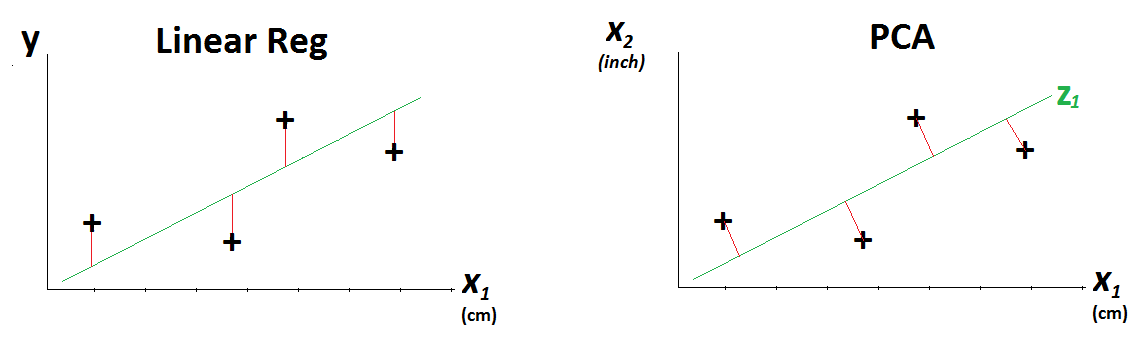
\includegraphics[totalheight=3 cm]{fig7.png}\caption{}
\end{figure}
\end{itemize}

\begin{itemize}
\item PCA algorithm
\begin{enumerate}
\item Compute 'covariance matrix' $\Sigma = \frac{1}{m} \sum_{i=1} ^m (x^{(i)})(x^{(i)})^T $,\\
where $x^{(i)}$ is $(n \times 1)$, and $\Sigma$ is $(n \times n)$\\
\item Compute 'eigenvectors' of matrix $\Sigma$

\begin{tcolorbox}
\begin{python}
[U, S, V] =svd(sigma)
\end{python}
\end{tcolorbox}
'svd' (singular value decomposition) is a MatLab function outputing 3 matrices. \\
\begin{itemize}
\item $U$ is a $n\times n$ matrix:
\begin{align}
U = \left[ \begin{smallmatrix} . & . & . & & & & . \\ . & . & . & & & & . \\ u^{(1)} & u^{(2)} & u^{(3)} & & & & u^{(n)}   \\ . & . & . & & & & . \\ . & . & . & & & & . \end{smallmatrix} \right]
\end{align}
If we want to reduce the data to $k$ dimensions, we take the 1st $k$ column vectors $(u^{(1)}, u^{(2)}, .., u^{(k)}) = U_{\text{reduce}} (n \times k)$.
\begin{align}
z^{(i)} = U_{\text{reduce}} ^T x^{(i)}
\end{align}
where $z^{(i)} \in \mathbb{R}^k$

\item Vectorized implementation of $\Sigma$ with $X = \left[ \begin{smallmatrix} --- (x^{(1)})^T ---\\-----\\ ------\\--- (x^{(m)})^T ---  \end{smallmatrix} \right]$
\begin{tcolorbox}
\begin{python}
Sigma = 1/m * (X' * X)
[U, S, V] = svd(Sigma)
Ureduce = U(:,1:k)
z = Ureduce' * X
\end{python}
\end{tcolorbox}
\end{itemize}
Remember that for PCA $x^{(i)} \in \mathbb{R}^n $ (without $x_0=1$ by convention)
\end{enumerate}
\end{itemize}

\subsubsection{Reconstruction from compressed representation}
\begin{align}
x_{\text{approx}} = U_{\text{reduce}} * z
\end{align}
$U_{\text{reduce}}$ is $(n \times k0$ and $z$ ($k \times 1)$ $\Rightarrow$ $x_{\text{approx}}$ is $\mathbb{R}^n$ 
\begin{figure}[H]
	\centering
        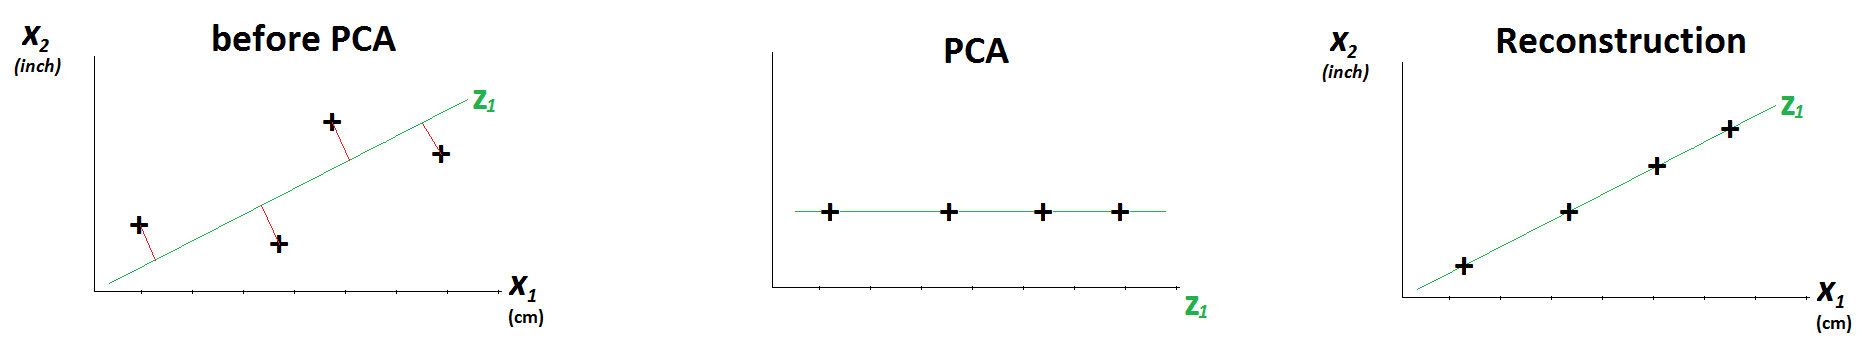
\includegraphics[totalheight=3 cm]{fig8.png}\caption{}
\end{figure}

\subsection{Choose the number of principal components}
\begin{itemize}
\item PCA minimizes Average Squared Projection Error:\\
\begin{align}
\frac{1}{m} \sum _{i=1} ^m || x^{(i)} - x_{\text{app}}^{(i)}||^2
\end{align}
\item Total variation in the data:\\
\begin{align}
\frac{1}{m} \sum _{i=1} ^m || x^{(i)} ||^2
\end{align}
\end{itemize}
Typically, choose $k$ to be the smallest value so that:
\begin{align}
\frac{\frac{1}{m} \sum _{i=1} ^m || x^{(i)} - x_{\text{app}}^{(i)}||^2}{\frac{1}{m} \sum _{i=1} ^m || x^{(i)} ||^2
} \leq 0.01 (or 0.05, 0.1)
\end{align}
which is interpreted as '99\% (95, 90) of the variance is retained'.
\begin{itemize}
\item Implementation
\end{itemize}
\begin{tcolorbox}
\begin{python}
Iteration
	Try PCA with k =1,
		Compute Ureduce, z[1], z[2], ..., z[m]
		                 xapp[1], xapp[2], ..., xapp[m]
		Check if Ratio of AverSquareProjection/TotalVariance <= 0.01
		k = k+1
\end{python}
\end{tcolorbox}

This can be achieved with $S$-vector output by svd MatLab function. $S$ is a diagonal matrix $n \times n$:
\begin{align}
S = \left[ \begin{smallmatrix} S_{11} & 0& 0&.. &0 \\ 0 & S_{22}& 0&.. &0 \\ . & .& .&.. &. \\. &.& .&.. &. \\. &.& .&.. &.\\ 0 & .& .&.. &S_{nn} \end{smallmatrix} \right]
\end{align}
For a given value of $k$:
\begin{align}
1- \frac{\sum_{i=1} ^k S_{ii}}{\sum_{i=1} ^n S_{ii}} \leq 0.01
\end{align}
for 99$\%$ of variance retained (which is a measure of the projection error).

\section{Advice for applying PCA}
\subsection{applying PCA for supervised learning speedup}
\begin{itemize}
\item inputs
Assume a dataset $\{(x^{(1)},y^{(1)}), ....,(x^{(m)},y^{(m)})  \}$.\\
Let's say $x^{(i)} \in \mathbb{R}^{10000}$ (which is often found in computer vision where images coudl be (100x100)px.
\item Extract inputs:\\
\begin{itemize} 
\item Unlabeled dataset  $\{x^{(1)}, ....,x^{(m)}  \} \in \mathbb{R}^{10000}$.
\item Apply PCA
\item $\{z^{(1)}, ....,z^{(m)}  \}$
\end{itemize}
\item New training set: $\{(z^{(1)},y^{(1)}), ....,(z^{(m)},y^{(m)})  \}$
\end{itemize}

\begin{itemize}
\item Note: Mapping (Ureduce) $x^{(i)} \rightarrow z^{(i)}$ should be defined by running PCA only on the training set. This mapping can then be applied as well to the examples $x_{cv} ^{(i)}$ and $x_{\text{test}} ^{(i)}$ in the cross validation and test sets.
\end{itemize}

\subsection{Application of PCA}
\begin{itemize}
\item Compression application:
\begin{itemize}
\item Reduce memory/disk need to store data
\item speed up learning algorithm
\end{itemize}
Choose $k$ using \% of variance retained.
\item Visualization application: 
$k$ is typically 2 or 3
\end{itemize}
\begin{appendices}

\section{Cost function versus iteration}

\begin{figure}[H]
	\centering
        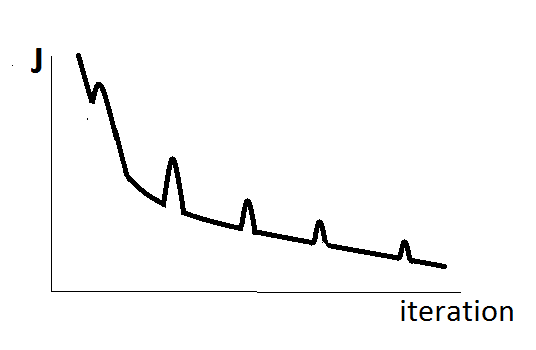
\includegraphics[totalheight=6 cm]{fig3.png}\caption{$J$ vs. iteration : It's not possible for the cost function to sometime increase. There must be a bug in the code.}
\end{figure}

\end{appendices}
\end{document}